\documentclass{article}
\usepackage[utf8]{inputenc}
\usepackage[margin=1in]{geometry}
\usepackage{tikz}

\tikzset{vx/.style={inner sep=1.7pt, outer sep=0pt,circle, fill}}
\tikzset{edge/.style={color=black,line width=.5}}


\title{Math Clinic Status Update 1}
\author{Team 1: Komi Agbo, Dalton Burke, Nick Mako, James Vance}
\date{October 28th, 2019}

\begin{document}

\maketitle

\section{Since our last update...}
We have completely changed our approach to the problem. Instead of thinking of
the problem as a Vehicle Routing Problem, where the order of deliveries directly
effects the cost of the route, our team noticed that how much the landfills and
storage locations are visited nearly eliminates this ordering constraint.

If customers only ever wanted container switches, the problem would be much
simpler. Where should the truck come from that's going to deliver the new
container? The nearest landfill. And where should the truck go after picking up
the full container? The nearest landfill. Filling the route with this data, we
end up with several \emph{stars}, each landfill being a center, and the points
surrounding it being the job sites. To service each star, you can take the jobs
in any order, the resulting cost will be the same. This will give us a lot of
leniency when trying to satisfy the constraints. The only task remaining is to
sew them together into routes for the drivers.

\begin{center}
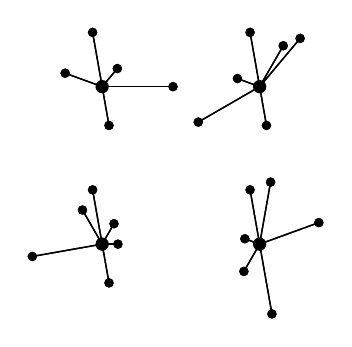
\begin{tikzpicture}
  \foreach \y in {0,2} {
    \foreach \x in {0,2} {
      \draw (\x,\y) node[vx]{};
    }
    \draw[edge] (0,0) -- ++(280:.5) node[vx, inner sep=1.2pt]{};
    \draw[edge] (0,0) -- ++(100:.7) node[vx, inner sep=1.2pt]{};
    \draw[edge] (0,0) -- ++(190:.9) node[vx, inner sep=1.2pt]{};
    \draw[edge] (0,0) -- ++(00:.2) node[vx, inner sep=1.2pt]{};
    \draw[edge] (0,0) -- ++(60:.3) node[vx, inner sep=1.2pt]{};
    \draw[edge] (0,0) -- ++(120:.5) node[vx, inner sep=1.2pt]{};

    \draw[edge] (0,2) -- ++(280:.5) node[vx, inner sep=1.2pt]{};
    \draw[edge] (0,2) -- ++(100:.7) node[vx, inner sep=1.2pt]{};
    \draw[edge] (0,2) -- ++(0:.9) node[vx, inner sep=1.2pt]{};
    \draw[edge] (0,2) -- ++(50:.3) node[vx, inner sep=1.2pt]{};
    \draw[edge] (0,2) -- ++(160:.5) node[vx, inner sep=1.2pt]{};

    \draw[edge] (2,2) -- ++(280:.5) node[vx, inner sep=1.2pt]{};
    \draw[edge] (2,2) -- ++(100:.7) node[vx, inner sep=1.2pt]{};
    \draw[edge] (2,2) -- ++(210:.9) node[vx, inner sep=1.2pt]{};
    \draw[edge] (2,2) -- ++(50:.8) node[vx, inner sep=1.2pt]{};
    \draw[edge] (2,2) -- ++(160:.3) node[vx, inner sep=1.2pt]{};
    \draw[edge] (2,2) -- ++(60:.6) node[vx, inner sep=1.2pt]{};

    \draw[edge] (2,0) -- ++(280:.9) node[vx, inner sep=1.2pt]{};
    \draw[edge] (2,0) -- ++(100:.7) node[vx, inner sep=1.2pt]{};
    \draw[edge] (2,0) -- ++(240:.4) node[vx, inner sep=1.2pt]{};
    \draw[edge] (2,0) -- ++(80:.8) node[vx, inner sep=1.2pt]{};
    \draw[edge] (2,0) -- ++(160:.2) node[vx, inner sep=1.2pt]{};
    \draw[edge] (2,0) -- ++(20:.8) node[vx, inner sep=1.2pt]{};
  }
\end{tikzpicture}\\
Stars
\end{center}

Customers can request drop-offs as well as pick-ups, with this, there are
some opportunities for extra optimization. A driver can drop off a container,
then, with the empty truck, go complete a pickup, without having to visit the
landfill. A driver completing a route like this (landfill $\rightarrow$ drop-off
$\rightarrow$ pick-up
$\rightarrow$ landfill) makes a \emph{triangle}, hence our name for this style, triangle
method.

\begin{center}
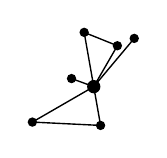
\begin{tikzpicture}

  \draw (0,0) node[vx]{};
    \draw[edge] (0,0) -- ++(280:.5) node[vx, inner sep=1.2pt]{};
    \draw[edge] (0,0) -- ++(100:.7) node[vx, inner sep=1.2pt]{};
    \draw[edge] (0,0) -- ++(210:.9) node[vx, inner sep=1.2pt]{};
    \draw[edge] (0,0) -- ++(50:.8) node[vx, inner sep=1.2pt]{};
    \draw[edge] (0,0) -- ++(160:.3) node[vx, inner sep=1.2pt]{};
    \draw[edge] (0,0) -- ++(60:.6) node[vx, inner sep=1.2pt]{};

    \draw[edge] (280:.5) -- (210:.9);
    \draw[edge] (60:.6) -- (100:.7);
\end{tikzpicture}\\
Triangles
\end{center}

A big question comes to mind, how do we choose the best triangles? Certainly,
some are better than others. To make this decision, we can construct a bipartite
graph, one set containing the drop-offs, and the other containing pick-ups, and
the existence of an edge between a drop-off and pick-up means that they are
\emph{compatible} (their constraints can work together). The
weight of the edge between a drop-off and a pick-up is calculated as the
difference between doing each normally (star method) and doing them combined as
a triangle. In this graph, a matching pairs up drop-offs and pick-ups to be
completed as a triangle. A minimum matching in this graph gives us the best
possible choice of triangles in order to make the route take the least amount of
time. Minimum matchings are extremely easy to compute (at least, compared to
traveling salesman type problems), our plan is to use the Hungarian Algorithm.

\begin{center}
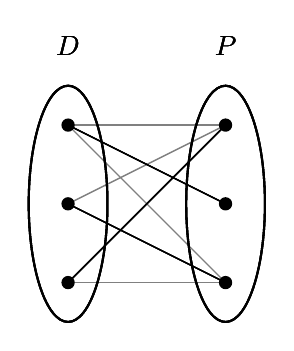
\begin{tikzpicture}
    \draw[edge, color=black!50] (0,1) -- (2,1);
    \draw[edge, color=black!50] (0,3) -- (2,1);
    \draw[edge, color=black!50] (0,3) -- (2,3);
    \draw[edge, color=black!50] (0,2) -- (2,3);

  \foreach \y in {1,2,3} {
    \foreach \x in {0,2} {
      \draw (\x,\y) node[vx]{};
    }
    \draw[line width=.75] (0,2) ellipse (.5 and 1.5);
    \draw[line width=.75] (2,2) ellipse (.5 and 1.5);
    \draw (0,4) node{$D$};
    \draw (2,4) node{$P$};

    \draw[edge] (0,1) -- (2,3);
    \draw[edge] (0,2) -- (2,1);
    \draw[edge] (0,3) -- (2,2);
  }
\end{tikzpicture}\\
An example matching
\end{center}

\section{What's on our plate now...}
\begin{itemize}
  \item Writing some basic code for the star case
  \item Working out some more details for
    \begin{itemize}
      \item Choosing transitions between landfills
      \item Satisfying constraints
      \item Using Delivery-Pickup strings as transitions (when they are more
        optimal than normal transitions)
    \end{itemize}
\end{itemize}
\section{What's next...}
\begin{itemize}
  \item Write more integration with data from UI team
  \item Write D-P matching
  \item Work more with the details from the last section
\end{itemize}



\end{document}

